% Tomas Coufal xcoufa09@stud.fit.vutbr.cz
% Content of the Bachelor Thesis
%!TEX root = xcoufa09.tex

\chapter{Introduction}
\label{chap:Introduction}
In the past few years the term of Cloud computing resonates worldwide, and gains its popularity. There have been plenty of papers and articles written about it, and every large IT corporation interested in this new market has brought their own solution. Cloud computing has become a well established business, and ultimate answer for nearly every demand for IT infrastructure these days. But when it comes to the meaning of these two words, not everyone knows what exactly to expect. In a nutshell, it means a highly scalable and accessible platform, reachable through a network connection. The word platform in this definition stands for a huge variety of software: from virtual machines and specialized databases to applications like web office suites. In so called \emph{Cloud}, whole internal corporate infrastructures are run along with end-user facing products with ease. Rising complexity and competition between different cloud providers and types of services, creates a demand for an easier management, providing more efficient yet reliable ways to ensure the same level of control over offered services.

In this thesis we describe the main challenges that cloud managing tools are facing while integrating with providers of various capabilities and including different systems and subsystems. The described process is going to be based on a real example, an implemented process of \textbf{IBM SoftLayer} cloud service integration into an open-source project, \textbf{ManageIQ}. This work covers how to distinguish and differentiate the same functionality across naming conventions and service capabilities, how to integrate them into \textbf{ManageIQ} and how to establish working communication between \textbf{IBM SoftLayer} and the cloud manager. This thesis also aims to simplify, sort out and sum up the knowledge needed to implement such integration for future \textbf{ManageIQ} provider integrators.

\section{Cloud computing}
\label{sec:Cloud computing}
Before we reveal the complexity of \emph{Cloud computing} and describe the challenges in managing cloud services across providers, it is worth describing what the word \emph{Cloud} actually stands for, why it is a need for huge variety of companies, and how the IT industry invented such technologies~\cite{cervone}.

\subsection{Transition from traditional computing to the cloud}
\label{sub:Transition from traditional computing to the cloud}

In history, the general approach to implementing a solid and reliable IT infrastructure has changed several times. To understand well the thought process behind this evolution, let me shortly describe the needs and demands of the industry.

\subsubsection{Traditional way}
\label{subs:Traditional way}

The historically first and simplest approach for a company to implement and manage their own service is to use their own machines and servers. To lower the risks of a hardware failure this solution requires to mirror the application and it's data over multiple servers or even into a cluster of serves. This brings a lot of investments and requires a lot of maintenance on the company's side.

Servers are considered a base unit that encapsulates all the necessary hardware, operating systems, storage, and any other utilities necessary. When the application reaches limits of its dedicated server, some additional hardware has to be provided. Despite the fact that an application can consume a lot of resources, it's not happening all the time. As an example, you can think of a delivery or ordering system. During the year the amount of transactions are equal but before e.g. Christmas the peak in transactions can be high. Nevertheless the downside is, once you have the server configured to run one application that can use all its resources during the peak, you can't utilize the resources left unused when the application is idle. Additionally, when the system encounters a failure, the recovery process is complicated. In the matter of scalability this approach is not functional enough.

\subsubsection{Virtualized computing}
\label{subs:Virtualized computing}

Because of all the disadvantages listed above, a new approach needs to be invented. To lower the complexity of hardware scaling, IT industry moved towards an increase in software difficulty. Unlike hardware maintenance, this can be automated easily and requires less resources to deploy. Servers are no more considered atomic units. The fact that hardware itself can be abstract leads to an invention of \emph{Virtualized computing}. The paradigm of virtualization presents a virtual machine manager also known as a \emph{Hypervisor}. This is a specialized operating system designed to run multiple operating systems as applications. This manager provides the necessary layer that can encapsulate each environment. The isolation of hardware from operating systems makes it possible to run multiple services on one physical machine. Each virtual machine is provided by the resources it demands and when these are left unused, the hypervisor manages to pass them where they are needed.

However, when a physical failure appears, the situation remains unchanged. The service has to be moved to another device. What differs is the solution. Usually, hypervisors are run in clusters of physical servers where they can cooperate. When one hypervisor is facing a hardware failure, the services are smoothly swapped to another physical device managed by a different hypervisor within the same cluster. This can happen without any outage of service and without the need for running a parallel fallback machine. This flexibility also helps the scalability mentioned above. In the case of multiple services running on one physical device, the resources are assinged dynamically. And in a case when an application demands more resources than the hypervisor can offer, the less loaded virtual machines are transitioned to another server within the cluster. This creates an environment where no virtual machine suffers from a significant lack of resources.

\subsubsection{Outsourcing virtualization}
\label{subs:Outsourcing virtualization}

The core idea behind virtualization is the same for \emph{Cloud Computing} as well. A company using a virtualized solution typically owns the physical servers and maintains them on their own. This produces much overhead costs. On the other hand in a \emph{Cloud Computing} environment, there is no need to insist on keeping and housing the infrastructure by a company. The operational responsibilities are shifted to the cloud provider who is now responsible for all the hardware and its maintenance. Providers offer remotely controlled virtual environments, location independent and highly scalable solutions. Advantages of virtual computing sustain, applications are still run in a virtual environment, scaled on demand and flexible. The creation of new virtual machines is a matter of minutes or less and no additional resources are needed.

\emph{Cloud Computing} providers usually implement a pay-as-you-go model where all costs are based on actual usage and new appliances are purchased when needed. Advantage of this payment model becomes even more significant when the company has a lot of applications that need to be run concurrently and their transaction peaks are expected at the same period of time. Cloud providers dispose with load balancing mechanisms and thanks to size of their clusters, the availability of the application is always guaranteed. The actual costs still remain much lower compared to the situation when a company has to provide all the hardware on their own. When the peaks diminish, all the necessary additional resources can be reused by the cloud provider for other applications. The same situation in the virtual computing model would lead to a state where these resources would be left unused on the company side. The idea of shared resources in huge clusters is one of the strongest advantages of cloud computing.

\subsection{Cloud typology}
\label{sub:Cloud typology}

Among all the described advantages of \emph{Cloud Computing}, not only the scalability has to be taken into account. There are plenty of fields where the cloud solution excels in. For example the \emph{National Institute of Standards and Technology} of the USA defines cloud computing by these five most essential characteristics~\cite{hu}:

\begin{enumerate}
	\item On-demand self-service
	\item Broad network access
	\item Resource pooling
	\item Rapid elasticity
	\item Measured service
\end{enumerate}

On-demand self-service stands for a possibility for consumers to provision computing power (meaning server time, dedicated storage, etc.) as needed and without the necessity to interact with the service provider in person by any means. This allows the customer to avoid the risk of not being able to scale his appliances when there is any kind of outage in the preferred type of communication established between him and the provider.

Broad network access is a term used to describe availability over network via standard communication channels while not discriminating client devices by type or platform. The term is mainly used in context of private clouds where this idea goes slightly against the security principles these clouds are designed for. The main reason to involve broad network access is to make the infrastructure available also for remote workers and via tablets and smartphones.

Resource pooling is a criterion considering dynamic assignment and reassignment of resources to different customers based on their demand in a multi-tenant model of cloud service. These resources are location independent and the customer is neither in control nor has the knowledge of the exact location of the resources. Nevertheless the location can be revealed on a higher level of abstraction, on a country or data center scale.

Rapid elasticity presumes the resources are provisioned and released automatically. These actions are done in a short period of time and from the customer's point of view the capabilities available typically appear unlimited and any amount of resources can be up-scaled at any time.

Measured service is a term used for automatic control over cloud cluster resources in order to monitor, analyze, control, and optimize the usage. This mechanism provides additional transparency over the service for both the customer and the provider.

Cloud solutions have many shapes and forms in general~\cite{hassan}. To distinguish and differentiate between common types of the \emph{Cloud}, multiple points of view should be mentioned. One of the discerning criteria to be considered is the availability to purchase a different deployment model. There exist private and public clouds. \emph{Public Cloud} means the cloud infrastructure (not the appliances) is widely accessible by anyone. No matter if an organization or a person, anyone is able to use the service provided. The Amazon's \emph{AWS EC2}~\footnote{\url{http://aws.amazon.com/ec2/}}, \emph{OpenShift by Red Hat}~\footnote{\url{https://www.openshift.com/}},  \emph{OpenStack}~\footnote{\url{https://www.openstack.org/}}, Microsoft's \emph{Azure}~\footnote{\url{https://azure.microsoft.com/en-us/}} or \emph{Google Cloud Platform}~\footnote{\url{https://cloud.google.com/compute/}} can serve as an example of this type of cloud service.

When customers are using a \emph{Public Cloud}, they share the same infrastructure for their virtual machines. In contrast, there is a second option available. These, so called \emph{Private Cloud}s, are strictly used by one customer only, and they are based on a special contract between the cloud service provider and the customer. This provides additional options for control over the purchased infrastructure and more security advantages as well. Since there is no other user in that cloud, it minimizes the risk of any vulnerability, in the isolation of each application, being exploited.

Another option how to differentiate between available cloud solutions is by its level of abstraction: the service models. According to the service-oriented architecture, cloud computing providers offer three main types of service. These are (in stacking order) \emph{Infrastructure as a service}, \emph{Platform as a service} and finally \emph{Software as a service}.

\subsubsection{Infrastructure as a service (IaaS)}
\label{subs:Infrastructure as a service (IaaS)}

Firstly, there is the most low-level approach to providing services via cloud, providing base infrastructure. This reflects the need for customized setups which are trusted by customer. In this case the term of infrastructure stands for virtual machines or even bare metal ones. These are usually deployed based on an images built by customers themselves or generic ones which allow to quickly scale over predefined setups. Integrating a provider of this kind is the subject of this thesis.

\subsubsection{Platform as a service (PaaS)}
\label{subs:Platform as a service (PaaS)}

By utilizing a PaaS, a customer gains an environment that allows him to develop and run his own applications without the need for building and maintaining a complex infrastructure. Such customer has access to a solid, stable and reliable platform of his desire and focus solely on the application he develops and deploys. The described environment offers countless setups and frameworks with or without included databases, continuous integration, etc. This approach brings the advantages of rapid, easy and secure deployment, along with other benefits of the cloud.

\subsubsection{Software as a service (SaaS)}
\label{subs:Software as a service (SaaS)}

The most advanced and complex level of abstraction in cloud computing. \emph{Software as a service} usually provides end-user facing applications accessible on demand. The provider installs and operates an application software for the customer in their cloud. Typically \emph{SaaS} is licensed on a subscription basis offering parametrized environment, along with high availability insurance. Great examples of such kind of service are \emph{Salesforce}~\footnote{\url{https://www.salesforce.com/}} and web office suites like \emph{Google Docs}~\footnote{\url{https://docs.google.com/}} or \emph{Microsoft Office 365}~\footnote{\url{http://office.microsoft.com/}}. The portfolio of services covered by SaaS is huge and wide beyond imagination. From offering solutions supplying different kinds of analyses like social networks profiling tools and advertisement, over communication platforms including video, audio, mailing services etc., to mobile offices like the ones mentioned above.

\section{IBM Cloud}
\label{sec:IBM Cloud}

Among others, the IBM company also offers their own cloud solution, the so called \textbf{IBM Cloud}. It's not a standalone project, it's a summary name for a whole portfolio of products. It comprises of complementary yet independent platforms and tools covering an extensive amount of application and use-cases delivering adjustable setups and products to the customer. When the customer demands IaaS, \emph{IBM SoftLayer} is the product he's asking for. For platform-based requirements, IBM offers a cloud service named \emph{Bluemix}. There is also a vast amount of SaaS solutions delivered by the company via their very own \emph{IBM cloud} market. Some of them based on the \emph{IBM Watson} intelligence, some standalone. This complex tooling allows IBM to deliver in the cloud market environment.

\chapter{IBM SoftLayer}
\label{chap:IBM SoftLayer}

This IaaS cloud service provided by IBM Company is one of the world's largest cloud services available. In order to integrate this provider of cloud infrastructure it's better to acknowledge and recognize the merit. Exploring and studying its parts and internal structure helps to understand the way to a successful integration. The very next step is to identify and describe the ways how the provider can be accessed via APIs and cloud binding libraries and what are the benefits or drawbacks of each option available. Finally, by comparing these approaches, it's necessary to objectify which one is the most suitable for our needs of integration into \textbf{ManageIQ}.

\section{Components}
\label{sec:Components}

Before elaborating on the cloud bindings it is necessary to introduce and describe the main and most important areas of IaaS clouds, with focus on the \textbf{IBM SoftLayer}. The most notable parts that are required to understand are listed below. Each user deploying his machine in cloud needs to decide on the following:

\begin{itemize}
	\item Where to place the machine?
	\item How is the virtualization encapsulated?
	\item What are the resources available for the purchased instance?
	\item Which software, operating systems are run and how to preserve data?
	\item How are the machines connected one to another?
\end{itemize}

Understanding these topics is essential for a customer to be able to successfully and effectively deploy his appliance.

\subsection{Regions, Zones and Data centers}
\label{sub:Regions, Zones and Data centers}

One of the most important yet changing parts when setting up the cloud infrastructure is to distinguish where the appliance is physically run (approximately). This is important in a case when customer wants to mirror his infrastructure around the globe with purpose to ensure its accessibility and reliability. It's a factor that can easily eliminate or at least reduce the connection issues caused by Internet service providers and exchange points outages. In other words, the application's swiftness is as good as it is possible and not dependent on its user's geographical location and time. Since neither the customer nor cloud provider is responsible and in control over the connectivity provided to users, placing customer's devices as close as possible to its end-user destination makes sense. This is what usually the \emph{Regions} are referring to. However, in a cloud environment the specification of the exact physical location is not dogmatic. The approximate and relative location is sufficient and the most common way is to refer to a continent or a market. For example the \textbf{Google Compute Engine}~\cite{gce} specifies its regions as: \texttt{Central US}, \texttt{Eastern US}, \texttt{Western Europe}, etc.

On the other hand a complementary entity takes place within each region. These are called \emph{Zones} or \emph{Availability Zones}. Numerous zones are present in each \emph{Region}. Each one is independent of another. The reason is to ensure that in a case of outage, scheduled maintenance or any other kind of issue affecting a zone the others are left untouched and available. When one zone is failing the others in the same region remain available and reliable.

By using and specifying proper \emph{Regions} and \emph{Availability Zones}, the customer can ensure and enhance reliability of his services, reduce latency and build a robust system which is both as close as the customer needs and distributed around the world in the same time. Each cloud provider has a slightly different philosophy of how they comprehend and implement these principles. Let's describe the two most common approaches.

We already mentioned the \textbf{Google Compute Engine} where the understanding of the area specifications is probably the most fitting the definition. There are \emph{Regions} which refer to a continent or a country where the data centers are placed. Also, within each of them there are a couple of \emph{Availability Zones}, usually 3 or 4 of them, and these are independent.

As a second example the \textbf{Microsoft Azure} provider can be mentioned. Their understanding of this scheme is a bit different. They provide a \emph{Region} based solution only~\cite{azure}. These are specified in much greater detail then in Google's case and there exist more of them as well. This provider is substituting \emph{Zones} by making regions smaller so customers can easily target the end-user (by selecting not just the continent but even a specific country) and yet keep the backup instance in the closest region. As an example, this is a sample how the \emph{Regions} are named and where they are placed in the \textbf{Azure} cloud provider: \texttt{Central US} in Iowa, \texttt{North Central US} placed in Illinois or \texttt{Japan West} set in Osaka.

Let's focus on how the scheme of\emph{Regions} and \emph{Zones} works in the \textbf{IBM SoftLayer} cloud provider. Their model is quite similar to the \textbf{Microsoft Azure}. However, besides other differences they do not use the term of \emph{Region}. Instead, the \emph{Data Center} term is used. This term truly refers to an exact location (for each center, the exact city is told). The product pages describe locations where data centers are placed~\cite{softlayer_datacenters}, for instance such centers are: \texttt{Dallas 01}, \texttt{Dallas 09}, \texttt{Amsterdam 02}, \texttt{Washington, D.C. 01} or just \texttt{Paris}. As you noticed, there might be some redundancy within a location. When there are multiple data centers in one city, each affected data center is numbered.

Speaking in the matter of the scheme defined in previous paragraphs, it's definitely needed to fit these in. It's required to find a proper category, because the scheme is reflecting the principles implemented in \textbf{ManageIQ}.

At first, let's take a look at how the work flow goes for the \textbf{IBM SoftLayer}. When the user is provisioning a new appliance he needs to select a \emph{Data Center} of deployment. This is the same situation as when deploying into \textbf{Google Compute Engine}, where the customer has to select the \emph{Region}.

Another point of view is that when there are multiple data centers within one city (let's say in the same \emph{Region}) the situation is reminiscent to a state when the provider offers multiple \emph{Availability Zones} for the region. Such behavior is reflected especially by these essential competences:

\begin{enumerate}
	\item Data centers are in the same \emph{Region}.
	\item Each one is independent on another.
\end{enumerate}

This view can evoke in us the idea that \textbf{IBM SoftLayer} provider is actually offering \emph{Availability Zones} as well, and it is mixing them with \emph{Regions} and calls them \emph{Data Centers}.

On the other hand, each \emph{Data Center} is selectable. In other words, it is required to pick one of them and deploy the appliance there. But this view goes strictly against the presumed policy that zones are managed internally by the provider and the user is usually not able to select and specify which zone is being used for his device. And there's also another reason why the comparison of zones and data centers within the same location is not accurate. There's no internal connection (besides the name) to link a \emph{Data Center} to the others within the same city. The missing relation (via API or network, etc.) is finally the reason why to model every data center as a separate \emph{Region} and do not bother the user with a new layer, new construct, the \emph{Availability Zones}.

\subsection{Servers}
\label{sub:Servers}

Once the user figures out where he can run his appliances, it's worth discovering what is being provisioned and run. In the clouds of the \emph{IaaS} type, it is usually some kind of \emph{Server}. Previously it's been mentioned~\ref{subs:Outsourcing the virtualization} that the most common type of device is a \emph{Virtual Server}, but this is not the only commodity available. For numerous security reasons, some cloud providers offer the possibility to run such a virtual server in three types of environment. \textbf{IBM SoftLayer} provides all of them.

\subsubsection{Shared hardware}
\label{subs:Shared hardware}

To run a \emph{Virtual Server} on shared hardware is the cheapest variant. It is also suitable for most of the customer needs. When a customer does not demand any special treatment like enhanced security features or a specific type of hardware, this is the way to go. The provisioned virtual server is placed on a server within the \emph{Data Center} and under a \emph{Hypervisor}. This hypervisor also manages other appliances and does not differentiate between the customers, the owners of the virtual machines. Shared hardware means a shared environment in a sense of a communal hypervisor and a shared physical layer between users.

\subsubsection{Dedicated hardware}
\label{subs:Dedicated hardware}

The opposite option is to reserve \emph{dedicated hardware}. It's more expensive, but on the other hand more secure. By using a dedicated machine for appliances owned by one user only, it provides another layer to secure the data. Also, some providers can offer an option to let the user be responsible over the \emph{Hypervisor} too. In addition, running appliances on \emph{dedicated hardware} makes the customer in complete control over the leased infrastructure.

\subsubsection{Bare metal servers}
\label{subs:Bare metal servers}

There's also an option, offered only by a minority of companies, to use the cloud to provide so called \emph{bare metal servers}. This means a completely different approach than cloud is usually known for. If a user wants to keep his data super secure and isolated yet in a stable, reliable and affordable environment it's possible to order a specific physical rack and run the customer's server there. Basically, this approach resembles a kind of server housing with the benefits of the cloud.

\subsection{Hardware Flavors}
\label{sub:Hardware Flavors}

Once the customer knows where the virtual machine should be run and what kind of virtualization the deployed setup requires, it's worth choosing the hardware resources (no matter if virtual or physical). This specification involves aspects like the processor cores count and frequency, amount of memory available for the device, or how data are being stored (if they are stored on a local hard drive or available via network, what type of hard drive it should be, how many of them are attached, what should be their capacity etc.). All these properties can be specified manually and in special cases they are. However, the more common work flow is to store the favorite setups as \emph{Flavors}. Each cloud provider also offers some default ones. For example the Table~\ref{tab:IBM SoftLayer default Flavors} below describes the default \emph{Flavors} used in the \textbf{IBM SoftLayer} cloud.

\begin{table}[ht]
	\centering
	\caption{IBM SoftLayer default \emph{Flavors}}\label{tab:IBM SoftLayer default Flavors}
	\begin{tabular}{llrrrr}
		\toprule
		Identifier & Name                 & CPU cores & Memory (RAM) & Hard drives (HDD)     \\
		\midrule
		m1.tiny    & Tiny Instance        & 1         & 1\,GB        & 1 $\times$ 25\,GB     \\
		m1.small   & Small Instance       & 2         & 2\,GB        & 1 $\times$ 100\,GB    \\
		m1.medium  & Medium Instance      & 4         & 4\,GB        & 1 $\times$ 500\,GB    \\
		m1.large   & Large Instance       & 8         & 8\,GB        & 1 $\times$ 750\,GB    \\
		m1.xlarge  & Extra Large Instance & 16        & 16\,GB       & 1 $\times$ 1\,000\,GB \\
		\bottomrule
	\end{tabular}
\end{table}

\subsection{Images, Templates and Snapshots}
\label{sub:Images, Templates and Snapshots}

Purposes of \emph{Images} are to replicate a virtual server running in cloud, store setups or deploy preconfigured systems. Some cloud providers and managers use a term \emph{Template} instead. They can be created in two possible ways.

The provider can produce some basic images with operating systems based on the default installation setups adjusted to reflect the cloud specific features, configurations, etc. Such images can also provide preconfigured application setups or platforms. As has been said, these templates are usually prepared by the provider to facilitate initial setups for the customer. Of course a user can deploy such images on his own too. But since this type of templates contains a default configuration, it's much more convenient for the customer to be provided  with them.

There's also a second way how to create an image. There's a possibility to create a \emph{Snapshot} of a running virtual machine. It is a pretty essential feature for each cloud to prepare a setup and save it as a template for backup and redeployment purposes. The user usually wants to scale his infrastructure and distribute it around the world in different regions or providers. By producing snapshots of his running virtual machines or uploading his own preconfigured ones it's easy to preserve state, data and environment and deploy, copy the instance, elsewhere. These \emph{Images} and \emph{Snapshots} created by a customer can be flagged as private and available for his own use only, or there's also a possibility to make such \emph{Template} publicly available for other users of that cloud.

\subsection{Networking}
\label{sub:Networking}

Finally, the last of the remarkable areas of IaaS clouds --- networking of the appliances. While a customer is provisioning a virtual machine, this machine is normally a part of a greater infrastructure. Inside that complex system, its components need to be connected and linked with others. In order to achieve that, clouds and virtualized computing brings mechanisms of \emph{Virtual networks}. These networks are modeled to behave and to offer the same functionality as their physical equivalents. There are couple of essential network infrastructure components. A list of the ones provided by \textbf{IBM SoftLayer} follows.

\subsubsection{Network Port}
\label{subs:Network Port}

Each virtual server is provided with some network interfaces with their own name, MAC address, etc. They are usually called \emph{Metwork Ports}. They point to the network interface properties of the virtual machine but they are also propagated outside to the managing API and provider's service applications. Thanks to this propagation they can be dynamically modified via API or the tooling provided by the cloud provider.

\subsubsection{Cloud Networks and Subents}
\label{subs:Cloud Networks and Subents}

Each port can be connected to a virtual \emph{Cloud Network} or a \emph{Cloud Subnet} while they work the same as in the world of regular computer networks. They are provided by IP address ranges (so the device can be connected, receive a mapping to one of them), speed limits, etc. They can also be controlled by \emph{Firewalls}. However, the understanding of cloud networks and subnets is also different across providers.

For example, let's describe the meaning of cloud networks and how they work in \textbf{IBM SoftLayer}. Each virtual server is given access to the two default networks for the data center. It is a \emph{Private Cloud Network} and the \emph{Public Cloud Network}. They take place of a gate to different points of interest.

\emph{Private Cloud Network} connects the device to internal appliances within the data center. For instance, such device can mean network storage volumes or databases, etc. On the other hand, the \emph{Public Cloud Network} is a gateway to the outer world, outside the data center and the cloud. To be precise the cloud networks in this sense do not offer any routing capabilities, they work just as a label of the range of interests available (reachable resources) for the device. Inside these networks, \emph{Cloud Subnets} can be set up. The subnets behave like the real networks or subnets. A customer can specify IP ranges and all other parameters he needs. The amount of subnets in the same network is not strictly limited for this cloud provider.

\subsubsection{Network Router}
\label{subs:Network Router}

Apart from the attached devices and addresses each network needs its \emph{Network Router}. This router is not a physical device either. For each subnetwork (as they are defined in the \textbf{IBM SoftLayer}) exists exactly one such router. Usually they are given a name and IP address and the only use for them is to build a proper illusion of the real network. Each router can service multiple subnets as it is known from regular computer networking. Within each cloud network there can be multiple routers. However, the architecture used in \textbf{IBM SoftLayer} does not provide more complex hierarchy, more levels of subnetworks. On the contrary, any advanced networking is not very common for cloud infrastructures currently deployed and this flat approach is sufficient enough.

\section{API access}
\label{sec:API access}

For managing purposes each cloud provider has it's own web interface. Such a tool usually contains all needed functionality: visualization of leased devices and machines, networking adjustments, provisioning of new appliances, creating snapshots, viewing spendings and other billing information.

On the other hand, an API is needed once more advanced users want to automate their work flows or create scripts to handle some common tasks. There are numerous different libraries allowing a user to connect to the provider. In this case it is essential to focus on the \textbf{IBM SoftLayer} provider with respect to the needs and capabilities of \textbf{ManageIQ}.

\subsection{Standard REST API}
\label{sub:Standard REST API}

The standard way offered by provider is to use the \textbf{IBM SoftLayer}'s \emph{REST API}~\cite{restapi}. This extensive API offers a complete access to nearly all features of the cloud infrastructure. It is a low level standard defining how to communicate with the cloud, how to format requests and what responses should be expected etc. The major advantages of the API is in its complexity and independence on a programming language.

\subsubsection{User authentication}
\label{subs:User authentication}

When a user is managing the cloud services via web interface, the normal and most common way to identify himself is to use \emph{username} and \emph{password}. While using APIs, the situation is a bit different. Each cloud defines the way on their own. \textbf{Google Compute Engine}, for instance, requires to specify the project name, user email and then uses a special \emph{Google JSON key} which is basically a project specific certificate for the user. The \textbf{Amazon Web Services EC2} cloud uses a generated pair of \emph{Access key ID} and a \emph{Secret Access key}. Finally, when it comes to the \textbf{IBM SoftLayer}, there are two factors used for authentication. It involves the normal \emph{User ID} (a customer specific ID) and a specially generated \emph{Secret API key} for each of the customer's administrator.

\subsubsection{Language bindings}
\label{subs:Language bindings}

The described API is pretty basic and low level in the aspect of connection handling and abstract operations. For better integration of this API into user projects the derived libraries have been built upon it to offer bindings and object based interface for different programing languages. Since \textbf{ManageIQ} is written in \emph{Ruby} we should focus and elaborate on the libraries created for this programming language.

\subsection{Softlayer API for Ruby}
\label{sub:Softlayer-API}

First of them is a \emph{SoftLayer API} brought by the SoftLayer developers~\cite{softlayer_api}. This library provides a Ruby Gem package named \texttt{softlayer\_api}. However, because of the lack of proper structure and disorganized code, it is not easy to follow for beginners. All provided activities are available via one service and the naming conventions abide by the \textbf{IBM Softlayer} standards. This makes it a bit complicated in the matter of maintenance while the provider is being integrated with others. By using this library, each developer willing to maintain the code has to understand internal \textbf{IBM Softlayer} work flows. The example Code~\ref{code:softlayer_api} describes the basic usage of this library.

\begin{lstlisting}[language=Ruby,caption={Example code for the \texttt{softlayer\_api}},label=code:softlayer_api,float=htpb]
require "softlayer_api"

# Specify the provider and credentials
SoftLayer::Client.default_client = SoftLayer::Client.new(
  :username => "<username>",
  :api_key  => "<api_key>"
)
# Connect
account = SoftLayer::Account.account_for_client()

# Lookup all provisioned servers
account.servers

=> [<SoftLayer::VirtualServer:0x00000002090ec8
		  @softlayer_client=
			  <SoftLayer::Client:0x00000002124ce0
				# client details like used credentials, API, etc.
				>
		  @softlayer_hash=
		   	{ "domain"=>"example.com",
		      "fullyQualifiedDomainName"=>"centos.example.com",
		    	"hostname"=>"centos",
		    	"id"=>17784479,
		    	"maxCpu"=>1,
		    	"maxMemory"=>1024,
					# etc.
			  }
	 ]

# Get the first server and check its state
server = SoftLayer::VirtualServer.server_with_id(17784479)
server[:powerState]

=> 'Running'
\end{lstlisting}

\subsection{Fog the Ruby cloud service library}
\label{sub:Fog cloud library}

There's also a \texttt{fog-softlayer} gem, a \emph{Fog} library for this provider~\cite{fog-softlayer}. \emph{Fog} is a cloud service library for Ruby available for many different providers across market. This makes the Gem easily understandable and compatible with other providers. It is also much simpler to maintain the structure and follow a pattern of other providers already available in the \textbf{ManageIQ} which are also implemented via \emph{Fog}. This library also offers extensive documentation (for \emph{Fog} in general) and example code for the \texttt{fog-softlayer} covering the desired functionality.

To contrast the \texttt{fog-softlayer} with \texttt{softlayer\_api}, the services and objects are more structured here. They also offer standardized cloud naming conventions which make it easier to follow and maintain. Its structure corresponds with every other provider in \emph{Fog}. It is kept and managed via 5 basic services which can operate separately.

\begin{itemize}
	\item \verb|Fog::Account| accessing customer account's organization if it is grouped with others
	\item \verb|Fog::Compute| is the most important service allowing the user to control servers (monitoring, provisioning, deployment, creating snapshots and more)
	\item \verb|Fog::Network| offers bindings to manage cloud networks, subnets, routers, etc.
	\item \verb|Fog::DNS| for managing DNS records
	\item \verb|Fog::Storage| provides connection to \emph{Bluemix} storage service
\end{itemize}

Each of the services has its own purpose, but the most important in a sense of cloud management are the \verb|Fog::Compute| and \verb|Fog::Network|. By using just these two, the user can easily manage his running appliances and deploy new ones. The code sample~\ref{code:fog_compute} shows the basic work flow for listing running servers and how to provision a new one.

\begin{lstlisting}[language=Ruby,caption={Example work flow for Fog SoftLayer},label=code:fog_compute,float=htpb]
require "fog/softlayer"

# Specify the provider and credentials
options = {
  :provider => "softlayer",
  :softlayer_username => "<username>",
  :softlayer_api_key  => "<api_key>"
}

# Connect to the Compute and Network service
compute = ::Fog::Compute.new(options)
network = ::Fog::Network.new(options)

# Lookup all provisioned servers
compute.servers.all

=>   <Fog::Compute::Softlayer::Servers
    [ <Fog::Compute::Softlayer::Server
        id=17784479,
        name="centos",
        domain="example.com",
        fqdn="centos.example.com",
        cpu=1,
        ram=1024,
        # etc.
      >,
			# other servers
    ] >

# Get the first server and check its state
server = compute.servers.get(17784479)
server.state

=> 'Running'

# Provision a new instance from image
provison_options = {
    :flavor_id => "m1.small",
    :image_id  => "1394bf94-e4e5-43bf-90ec-5eedbdcc420d",
    :name      => "ubuntu",
		:domain    => "example.com",
    :datacenter => "ams01"
}
new_instance = compute.servers.create(provision_options)
new_instance.id

=> 17784894
\end{lstlisting}

\chapter{ManageIQ}
\label{chap:ManageIQ}

A project named \textbf{ManageIQ} is an open-source technology developed by a community supported and sponsored by the Red Hat company. This project aims to provide an easy management over cloud solutions across providers by offering comfortable import, appliances management, network links visualization allowing modifications, and infrastructure provisioning capabilities. Expectations are high since all integrated technologies are different considering functionality and capability. To cover those variations, \textbf{ManageIQ} provides abstract internal bindings that should suit most of the needs.

\section{Providers}
\label{sec:Providers}

\begin{figure}[ht!]
	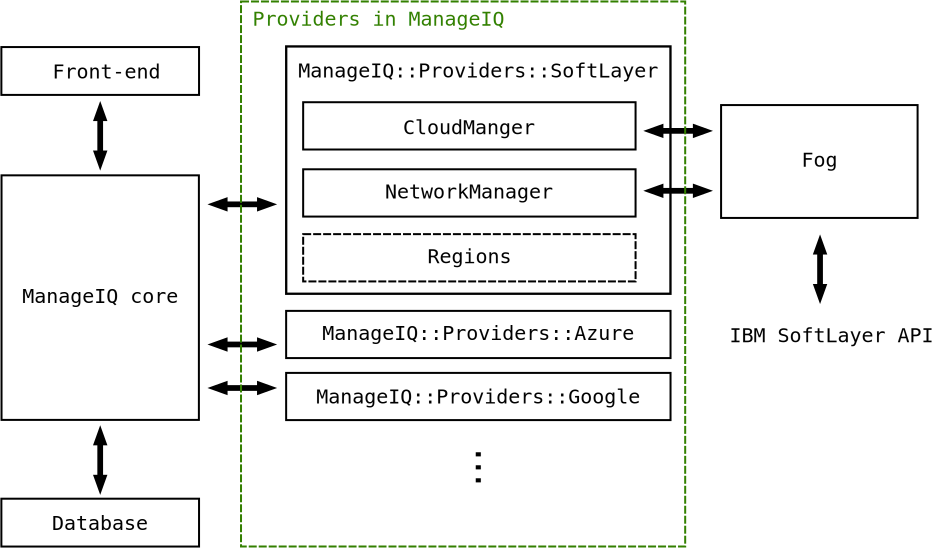
\includegraphics[width=\textwidth]{fig/architecture}
	\caption{Providers in \emph{ManageIQ}}\label{fig:Providers in ManageIQ}
\end{figure}

The Developer's guide~\cite{manageiq_dev} defines available bindings for each provider. Each provider is represented by a so called \emph{External Management System}. The reason for such name is mainly historic, today each provider offers a complex functionality which needs to be broken into smaller, separate managers. A Figure~\ref{fig:Providers in ManageIQ}  categorize the providers into the \textbf{ManageIQ}'s architecture . This reveals the overall picture how these managers are related with other parts of the framework. In the case of \textbf{IBM SoftLayer} these are the \emph{Cloud Manager} and the \emph{Network Manager}. Each of them is given it's namespace and can be derived from a base manager of that type. These managers cover, or try to cover these areas:

\begin{itemize}
	\item \emph{Inventory} for listing and tracking all the cloud properties
	\item \emph{Event Collection and Handling} for event driven work flows and dynamic system
	\item \emph{Metric Collection and Handling} for analysis over inventory objects, utilization etc.
	\item \emph{Provisioning and Orchestration} is adding features to dynamically deploy new setups in the provider
	\item \emph{Lifecycle} for managing the already deployed ones
	\item \emph{SmartState Analysis} is a low-level analysis tool for \emph{Virtual Machines} and \emph{Images}
\end{itemize}

Currently, due to missing features in the API for implemented provider we are able to cover just the \emph{Inventory}, \emph{Provisioning and Orchestration}, and \emph{Lifecycle} features.

In general, there exist three ways how to collect data about the provider:

\begin{itemize}
	\item \emph{Refresh Worker}
	\item \emph{Event Worker}
	\item \emph{Metric Worker}
\end{itemize}

Because of the reasons described above, we are currently able to implement and use just the first one of them, the \emph{Refresh Worker}. The properties imported by the refresh are listed and described below.

\section{Implemented Interfaces and Models}
\label{sec:Implemented Interfaces and Models}

\textbf{ManageIQ} uses a hierarchical scheme of models. While adding a new provider it is a \verb|ManageIQ::Providers| which has to be implemented. For \textbf{IBM SoftLayer} as a cloud provider there are 3 main parts, classes required:

\begin{itemize}
	\item \verb|"ManageIQ::Providers::Softlayer::CloudManager"| for the appliances management
	\item \verb|"ManageIQ::Providers::Softlayer::NetworkManager"| for networking
	\item \verb|"ManageIQ::Providers::Regions"| enlisting all available \emph{Regions}
\end{itemize}

Both of the managers inherit from their \emph{Base Manager}, for example, for the \emph{Cloud Manager} it is \verb|"ManageIQ::Providers::CloudManager"|. These managers implement the behavioral principles for \emph{Cloud Refresh} or event driven management purposes. In order to store connection bindings, which are common for both, there is a special \emph{Manager Mixin}.

These models are places in the \verb|app/models/manageiq/providers/<provider>| folder where \verb|<provider>| address the implemented provider. As this thesis describes the implementation of \textbf{IBM SoftLayer}, let's consider as a \verb|<provider_root>| the folder\\ \verb|app/models/manageiq/providers/softlayer|.

In the \verb|app/models/manageiq/providers/softlayer/| folder there can be found (the main components):

\begin{itemize}
	\item \verb|regions.rb| as a \emph{Regions} storage
	\item \verb|manager_mixin.rb| for the \emph{Manager Mixin}
	\item \verb|cloud_manager.rb| defining the \emph{Cloud Manager} behavior
	\item \verb|cloud_manager| folder containing all components required by the cloud manager
	\item \verb|network_manager.rb| containing the \emph{Network Manager}
	\item \verb|network_manager| folder with content required by the required by the network manager
\end{itemize}

The following sections describe each one of them.

\section{Connection Management}
\label{sec:Connection Management}

The connection is a common feature and requirement for both of the implemented managers. This connection handler is kept separated from them for easier maintenance. The class for that is called \emph{Manager Mixin}. This mixin also contains the basic \emph{Discovery} work flow which is described bellow in the Section~\ref{sec:Discovery}. But the main purpose of the mixin remains in establishing the connection via \emph{Fog}, verifying credentials and providing the manager with proper service. How to connect via \emph{Fog} to the \textbf{IBM SoftLayer} is described in the Code~\ref{code:fog_compute}.

\section{Regions}
\label{sec:Regions}

What \emph{Regions} are has already been described. However, for the integration purposes it's needed to understand how they are treated in the \textbf{ManageIQ}.

When a user is adding a new provider he has to specify the \emph{Region}. Basically, he is adding a \emph{Region} specific provider. This is a policy intended to keep the UI and the overall environment clean for the user. Imagine a situation where such a user has his devices deployed in many providers. In the case when all \emph{Regions} of each provider are added, his interface can be flooded by them. The other approach is to add one \emph{Region} per provider. And once the user needs to attach another one, he adds a new provider.

It is also required to list all available regions before a user connects to the provider. The application uses one step form for adding a provider, so he has to be able to specify the \emph{Region} before his credentials are proceed. And since every API client requires to authenticate before any actions can be done, it is required to list all regions statically in a file \verb|<provider_root>regions.rb|.

\section{Discovery}
\label{sec:Discovery}

The work flow described above can be slightly inconvenient when the user already has devices deployed in many different \emph{Regions}. For such situations, there is a \emph{Discovery} process. There, the user just specifies his credentials and the process does the work for him. The application places his discovery into a tasks queue and when the discovery proceeds, it iterates over every \emph{Region}. While there are \emph{Virtual machines} present in that region, it is registered as a new provider and its \emph{Refresh} is scheduled. This work flow is specified in the \verb|ManagerMixin| class.

\section{Cloud Manager}
\label{sec:Cloud Manager}

\emph{Cloud Manager} is a class specified for each provider and inherits from a base \verb|CloudManager|. In this case it is specified as \verb|ManageIQ::Providers::Softlayer::CloudManager|. It provides an interface over the cloud devices. The main purpose of this class is to cover all functionality needed to refresh and manage \emph{Virtual Servers} and every other aspect needed in order to provision and access them. All the links between devices are discovered separately and this class does not care about the internal representation of network components. Nevertheless, this manager maps the networking identificators of discovered devices into an internal database and once the networks are discovered, the system links them together.

All the entities and submodules described in this manager are populated by the \emph{Cloud Refresh}. There are also implemented relations and delegations for networking properties into the \emph{Network Manager}.

\clearpage
\subsection{Cloud Refresh}
\label{sub:Cloud Refresh}

To run a discovery service or refresh of the provider, the \emph{Cloud Refresh} namespace has to be defined. This is the most important class for each manager. It covers the import and mapping of every supported entity which is watched by the manager. The \emph{Refresh} procedure itself is defined and proceed in three separate phases:

\begin{itemize}
	\item \verb|:Refresher|
	\item \verb|:RefreshWorker| and \verb|:Runner|
	\item \verb|:RefreshParser|
\end{itemize}

This \emph{Refresh} is the base and most important back-end part of a new provider. It's main role is to fill the internal database with all inventory needed for further usage. The scheme that defines which attributes and inventory models are available is prescribed in the Developer's guide and documentation~\cite{manageiq_dev} in the \emph{Providers database architecture} and \emph{Provider Overview} guides.

\subsubsection{Refresher}
\label{subs:Refresher}

The \verb|:Refresher| specifies the work flow of the refresh. It tells the \textbf{ManageIQ} what refresh should be run, how to store all discovered appliances and which database schemes and tables should be affected. The major issue which this class takes care of is to identify which provider the devices belongs to. This refresher, when initiated, also queues a refresh of the providers \emph{Network Manager}.

\subsubsection{Refresh Worker}
\label{subs:Refresh Worker}

The worker is a specification of the way an import is handled. Normally, no modification to the standard process is required. It's the same for this provider. Each provider needs a \verb|:RefreshWorker| in order to register the run of refresh. The naming conventions and scheme of \textbf{ManageIQ} require also the \verb|:Runner| sub-class to be defined. Both of them inherit all the functionality from the base cloud manager's refresh worker.

\subsubsection{Refresh Parser}
\label{subs:Refresh Parser}

This class is the most important part of the refresh process. It defines which devices are added and where these should be registered in \textbf{ManageIQ}. Here, it is specified how the mapping of each of the following entities is done between the provider client library (in the case of \textbf{IBM SoftLayer} it is \texttt{fog-softlayer}) and the internal structure. The mapping (whether the device is \emph{Virtual Server} or \emph{Flavor} etc.\ and its properties) where to store these information is specified as well.

\clearpage
\subsection{Availability Zones}
\label{sub:Availability Zones}

As we elaborated in the Subsection~\ref{sub:Regions, Zones and Data centers}, there are no sufficient \emph{Availability Zones} present in \textbf{IBM SoftLayer}. On the other hand, each cloud manager requires a \emph{Zone} to be defined. To satisfy this need, a new default zone has been created. It does not affect any operation over the provider, although for the internal needs of the data hierarchy inside \textbf{ManageIQ}'s database it is present.

To preserve the naming conventions of \textbf{ManageIQ} even in this case, it is required to use two separate mapping functions. The first one, normally used to fetch data from the provider, now creates a list containing one element, the default zone. Then, it lets to parse it via the second function and store it into the designated place. The model for the zone uses a modified instance of \verb|Fog::Model| as the default zone~\ref{code:fog_model_zone}. This approach has been used instead of defining a special class for the zone because there is no need to have such a class available in the namespace. There is always going to be only one instance present in total and only during the refresh.

\begin{lstlisting}[language=Ruby,caption={Declaration of the default \emph{Availability Zone}},label=code:fog_model_zone,float=htpb]
# Create new fog model
default_zone = ::Fog::Model.new

# Inject methods for :name and :id to return default values for provider
{:name => @ems.name, :id => 'default'}.each do |method, value|
  default_zone.define_singleton_method(method) { value }
end

a_zones = [default_zone]
\end{lstlisting}

\begin{table}[ht]
	\centering
	\caption{\emph{Availability Zone} attributes mapping}\label{tab:Availability Zone attributes mapping}
	\begin{tabular}{ll}
		\toprule
		Attribute       & Corresponding value                                                              \\
		\midrule
		ID              & \verb|availability_zone.id.downcase|                                             \\
		\verb|:type|    & \small\verb|ManageIQ::Providers::Softlayer::CloudManager::AvailabilityZone.name| \\
		\verb|:ems_ref| & \verb|availability_zone.id.downcase|                                             \\
		\verb|:name|    & \verb|availability_zone.name|                                                    \\
		\bottomrule
	\end{tabular}
\end{table}

\subsection{Authentication Key Pairs}
\label{sub:Authentication Key Pairs}

Since \textbf{ManageIQ} aims to completely manage over different providers, besides monitoring purposes, it is essential to provide user with the possibility to connect to the machine. While there are any \emph{Authentication Key Pairs} attached to the device this is the class which takes care of them. Each key pair, when created, contains a name and a fingerprint. This provider specifies the key pair with a label as a name and a certificate as a fingerprint. Fetching \emph{Authentication Key Pairs} from the provider is easily done via \emph{Fog} by a simple run of \verb|compute.key_pairs.all| command.

\begin{table}[ht]
	\centering
	\caption{\emph{Authentication Key Pair} attributes mapping}\label{tab:Authentication Key Pair attributes mapping}
	\begin{tabular}{ll}
		\toprule
		Attribute           & Corresponding value                                                         \\
		\midrule
		ID                  & \verb|key_pair.id|                                                          \\
		\verb|:type|        & \small\verb|ManageIQ::Providers::Softlayer::CloudManager::AuthKeyPair.name| \\
		\verb|:name|        & \verb|key_pair.label|                                                       \\
		\verb|:fingerprint| & \verb|key_pair.key|                                                         \\
		\bottomrule
	\end{tabular}
\end{table}

\subsection{Flavors}
\label{sub:Flavors}

What \emph{Flavors} are was already discussed in Flavors~\ref{sub:Hardware flavors}. \emph{Fog} allows to list all available \emph{Flavors} via \verb|compute.flavors.all| command. The Code~\ref{code:fog_flavors}. All data available about the flavor are listed in plain format except the disk sizes. The total size has to be counted for each \emph{Flavor} separately by summing the sizes of all available disks.

\begin{lstlisting}[language=Ruby,caption={Sample of \emph{Flavors} data},label=code:fog_flavors,float=htpb]
# Fetch Flavors from SoftLayer
compute.flavors.first
=>   <Fog::Compute::Softlayer::Flavor
    id="m1.tiny",
    cpu=1,
    disk=[{"device"=>0, "diskImage"=>{"capacity"=>25}}],
    name="Tiny Instance",
    ram=1024
  >
\end{lstlisting}

\begin{table}[ht]
	\centering
	\caption{\emph{Flavor} attributes mapping}\label{tab:Flavor attributes mapping}
	\begin{tabular}{ll}
		\toprule
		Attribute              & Corresponding value                                                    \\
		\midrule
		ID                     & \verb|flavor.id|                                                       \\
		\verb|:type|           & \small\verb|ManageIQ::Providers::Softlayer::CloudManager::Flavor.name| \\
		\verb|:ems_ref|        & \verb|flavor.id|                                                       \\
		\verb|:name|           & \verb|flavor.id|                                                       \\
		\verb|:description|    & \verb|flavor.name|                                                     \\
		\verb|:cpus|           & \verb|flavor.cpu|                                                      \\
		\verb|:cpu_cores|      & \verb|flavor.cpu|                                                      \\
		\verb|:memory|         & \verb|flavor.ram * 1.megabyte|                                         \\
		\verb|:root_disk_size| & Counted separately, data taken from \verb|flavor.disk|                 \\
		\bottomrule
	\end{tabular}
\end{table}

\subsection{Virtual Machines}
\label{sub:Virtual Machines}

This is the most important commodity that has been imported and discovered. Each \emph{Virtual Machine} carries information about its name, domain, hardware configuration and even \emph{Flavor}, \emph{Image} which it is based upon or \emph{Authentication key pairs} attached. The attribute mapping is described in Table~\ref{tab:Virtual Machine attributes mapping}. Every attribute listed is successfully mapped except the \emph{Disks} discovery. The \emph{Softlayer API} described in the Subsection~\ref{sub:Standard REST API} provides every piece of information needed, except the effective disk size. Currently it's been decided to wait until the support for this value is in place. For now, no disks are mapped for any \emph{Virtual Machine} in this provider but the functionality is prepared so once these data are available, it can be easily updated.

Each \emph{Virtual Machine}, once mapped into the \textbf{ManageIQ}, offers an interface for its power management. This management also has to be binded to propagate the requests into the provider. This is done via the sub-class \verb|:VM| and its management modules \verb|:Operations::Power| and \verb|:Operations::Guest|. \textbf{IBM Softlayer} and \texttt{fog-softlayer} allows to:

\begin{itemize}
	\item Switch off the instance via \verb|instace.stop|
	\item Turn back on using \verb|instance.start|
	\item Reboot the appliance by \verb|instance.reboot|
	\item And finally terminate it by invoking the \verb|instance.destroy| command
\end{itemize}

Unfortunately \textbf{IBM SoftLayer} does not offer to \emph{Suspend}, \emph{Pause} or \emph{Hibernate} the instance.

\begin{table}[ht]
	\centering
	\caption{\emph{Virtual Machine} attributes mapping}\label{tab:Virtual Machine attributes mapping}
	\begin{tabular}{ll}
		\toprule
		Attribute                    & Corresponding value                                                \\
		\midrule
		ID                           & \verb|instance.id.to_s|                                            \\
		\verb|:type|                 & \small\verb|ManageIQ::Providers::Softlayer::CloudManager::VM.name| \\
		\verb|:uid_ems|              & \verb|instance.id.to_s|                                            \\
		\verb|:ems_ref|              & \verb|instance.id.to_s|                                            \\
		\verb|:name|                 & \verb|"#{instance.name}.#{instance.domain}"|                       \\
		\verb|:vendor|               & \verb|"softlayer"|                                                 \\
		\verb|:raw_power_state|      & \verb|instance.state|                                              \\
		\verb|:flavor|               & \verb|instance.flavor_id|                                          \\
		\verb|:operating_system|     & \verb|{:product_name => instance.os_code}|                         \\
		\verb|:availability_zone|    & Fetched the defaulf \emph{Availability Zone} from data storage     \\
		\verb|:key_pairs|            & Fetched from data storage                                          \\
		\midrule
		\multicolumn{2}{l}{Hash for \texttt{:hardware} information}                                              \\
		\midrule
		\verb|:cpu_sockets|          & \verb|instance.cpu|                                                \\
		\verb|:cpu_total_cores|      & \verb|instance.cpu|                                                \\
		\verb|:cpu_cores_per_socket| & 1                                                                  \\
		\verb|:memory_mb|            & \verb|instance.ram|                                                \\
		\verb|:disks|                & Not effectively populated                                          \\
		\bottomrule
	\end{tabular}
\end{table}

\clearpage
\subsection{Image Templates}
\label{sub:Image Templates}

In each \emph{Region}, there are specific \emph{Images} available. There are \emph{Public Images} created by other users or made publicly available by the cloud provider. Also, there are \emph{Private Images} created just for the needs of the customer. While importing them, we need to distinguish which images belong to what category. Also, there are other aspects that would be great to categorize. Unfortunately, this is not available via staging APIs. For example we would like to be able to categorize an image by operating system or designated and required disk space. It would also be helpful to differentiate which images are available for purchase and which are already old and their base operating system image is already missing. Currently, none of this functionality is available via API and just the basic data is accessible. Because of the defect mentioned above, the additional features have not been implemented. The mapping used for images can be seen below.

\begin{table}[ht]
	\centering
	\caption{\emph{Image} attributes mapping}\label{tab:Image attributes mapping}
	\begin{tabular}{ll}
		\toprule
		Attribute                  & Corresponding value                                                      \\
		\midrule
		ID                         & \verb|image.id|                                                          \\
		\verb|:type|               & \small\verb|ManageIQ::Providers::Softlayer::CloudManager::Template.name| \\
		\verb|:uid_ems|            & \verb|image.id|                                                          \\
		\verb|:ems_ref|            & \verb|image.id|                                                          \\
		\verb|:name|               & \verb|image.name|                                                        \\
		\verb|:vendor|             & \verb|"softlayer"|                                                       \\
		\verb|:tempalte|           & \verb|true|                                                              \\
		\verb|:publicly_available| & \verb|image.public?|                                                     \\
		\bottomrule
	\end{tabular}
\end{table}

\subsection{Tags}
\label{sub:Tags}

One of the most important aspects of \textbf{ManageIQ} is the capability to \emph{Tag} user's devices across providers and types. \textbf{IBM SoftLayer} also offers tagging capabilities. Each virtual machine can be tagged and labeled, and multiple labels can be applied on the device. The same can be said about the \textbf{ManageIQ}. However, this provider offers such functionality just for provisioned appliances, but not for other types of devices like \emph{Cloud Networks}, \emph{Network Routers} or \emph{Images}. This makes the import of tags from provider less efficient. There's also another problem that blocks the correct usage of tags in the cloud manager.

The issue is that \textbf{ManageIQ} currently does not offer a way to propagate tag changes into the provider. So, in a situation when a user modifies tags of a server in the cloud manager and then wants to refresh the provider, old \emph{Tags} are imported again and his changes are overwritten. Due to this fact, the tags are currently being ignored and skipped during refresh and discovery.

\clearpage
\subsection{Provision}
\label{sub:Provision}

The default provision model used in \textbf{ManageIQ} is \emph{Cloning}. But it does not refer to cloning in a sense of replicating an already available instance. It is used for the \emph{Image} deployment into a new \emph{Virtal Machine}.
The work flow basically follows the standard form used by the \texttt{fog-softlayer} seen in the Code~\ref{code:fog_compute}. The user selects the desired \emph{Image}, specifies \emph{Flavor}, \emph{Cloud Subnetworks} via web UI and declares the name and domain to use for the newly created device.

The code in the back-end then processes user input and based on his selection, prepares a \verb|cloning_options| hash. The source code bellow describes a function to prepare such data for \textbf{IBM Softlayer}.

\begin{lstlisting}[language=Ruby,caption={Prepare cloning options},label=code:cloning,float=htpb]
def prepare_for_clone_task
  clone_options = super
  ems = source.try(:ext_management_system)
  vlan_id = get_option(:cloud_network)
  # NOTE: Private vlan is represented in the provisioning form
	# as a :cloud_subnet (rendered as a same type so there's no
	# need for a new specialized field)
  private_vlan_id = get_option(:cloud_subnet)

  # NOTE: Cloning might fail for some images due to missing base
	# OS (in the image). This information is not available via API,
	# it's safe to use own images though.
  additional_options = {
    :flavor_id    => instance_type.name,
    :image_id     => source.uid_ems,
    :name         => dest_name,
    :domain       => get_option(:vm_domain),
    :datacenter   => ems.provider_region,
    :vlan         => find_cloud_network_in_vmdb(vlan_id),
    :private_vlan => find_cloud_network_in_vmdb(private_vlan_id),
  }

  clone_options.merge(additional_options)
end
\end{lstlisting}

\clearpage
\section{Network Manager}
\label{sec:Network Manager}

In order to connect and visualize relations of discovered devices, \textbf{ManageIQ} brings the class \verb|NetworkManager|. A separate \emph{Network Manager} is currently a new feature included in \textbf{ManageIQ}. The \textbf{IBM Softlayer} is one of the first providers adapting this structure. The current implementation uses the \emph{Cloud Manager} as default for delegating some of the workload onto this manager. This manager has it's own refresh capabilities and the refresh and discovery is it's main purpose. Today, neither \textbf{ManageIQ}, nor \texttt{fog-softlayer} is capable of manipulating networks. This layer is static for display and monitoring purposes.

The main change in the process of connecting to the provider's API is using the \verb|Fog::Network| service instead of the \verb|Fog::Compute|. The connection to this service is made analogically as for the compute service so the following text is referring to the \verb|network| variable described at Code~\ref{code:fog_compute}.

\subsection{Network Refresh}
\label{sub:Network Refresh}

In the core, the purpose of \emph{Network Refresh} is the same as for the \emph{Cloud Refresh}. And the work flow is also the same: this refresh requires the same steps to be implemented (\verb|:Refresher|, \verb|:RefreshWorker|, \verb|:Runner| and \verb|:RefreshParser|). They provide the same role as has already been explained.

The \verb|:RefreshParser| is capable of exploration over:

\begin{itemize}
	\item \emph{Cloud Networks} and \emph{Cloud Subetworks}
	\item \emph{Network Ports}
	\item \emph{Network Routers}
\end{itemize}

Each component's discovery is initiated via a call to a corresponding function. In network discovery, these functions are registered: \verb|get_cloud_network|, \verb|get_network_ports|, \\ \verb|get_cloud_subnets\,(cloud_network)| and \verb|get_network_routers|.

\subsection{Cloud Networks}
\label{sub:Cloud Networks}

It's already been described how \textbf{IBM Softlayer} treats \emph{Cloud Networks}. They are used as labels without networking attributes, yet defining the connection and subnetwork purposes. There exist two types of such networks and a specific sub-class has been created for each of them:

\begin{itemize}
	\item \verb|:CloudNetwork::Public| for public networks that interface the Internet and outer connections outside of the data center.
	\item \verb|:CloudNetwork::Private| which purpose is to connect devices with each other and with network storage or any other internal service within the data center
\end{itemize}

\begin{table}[ht]
	\centering
	\caption{\emph{Cloud Network} attributes mapping}\label{tab:Cloud Network attributes mapping}
	\tabcolsep=4pt
	\begin{tabular}{ll}
		\toprule
		Attribute              & Corresponding value                                                         \\
		\midrule
		ID                     & \verb|cloud_network.id.to_s|                                                \\
		\verb|:type|           & \small\verb|"ManageIQ::Providers::Softlayer::NetworkManager::CloudNetwork"| \\
		                       & + suffix (\small{\verb|"::Private"|} or \small{\verb|"::Public"|})          \\
		\verb|:ems_ref|        & \verb|cloud_network.id.to_s|                                                \\
		\verb|:name|           & \verb|cloud_network.name| if present or a custom string                     \\
		                       & \verb|"Public"| (or \verb|"Public"|) \verb|"VLAN on <hostname>"|            \\
		\verb|:status|         & \verb|"active"|                                                             \\
		\verb|:cidr|           & \verb|nil|                                                                  \\
		\verb|:enabled|        & \verb|true|                                                                 \\
		\verb|:cloud_subnets|  & Initiated discovery and fetched the data from local storage                 \\
		\verb|:network_router| & \verb|cloud_network.router|                                                 \\
		\bottomrule
	\end{tabular}
\end{table}

\subsection{Cloud Subnetworks}
\label{sub:Cloud Subnetworks}

In case of \emph{Cloud Subnets} the situation is a bit more difficult. These networks are not directly displayed via \emph{Fog} like the other network components. However, both entities using and interfacing these subnetworks contain desired data. These two entities are \emph{Cloud Networks} and \emph{Network Ports}. Each of them provides enough data to register a subnet. It is considered a better practice while describing components to start from the greater picture to smaller parts. The \emph{Cloud Network} can be considered a bigger and more important component because it can contain more \emph{Network Ports} and represents a parent for each \emph{Cloud Subnet}.

While running a discovery over a \emph{Cloud Network}, all related subnetworks are discovered as well. This behavior is ensured by calling \verb|get_cloud_subnets(cloud_network)| during parsing action for each network. When all subnets are found, they are parsed, registered and stored in \textbf{ManageIQ}'s local storage. Later, when the refresh process reaches the \emph{Network Ports} discovery, their identificators are found and they can be located in the database and linked to the port.

\begin{table}[ht]
	\centering
	\caption{\emph{Cloud Subnetwork} attributes mapping}\label{tab:Cloud Subnetwork attributes mapping}
	\tabcolsep=1pt
	\begin{tabular}{ll}
		\toprule
		Attribute                 & Corresponding value                                                        \\
		\midrule
		ID                        & \verb|cloud_subnet.id.to_s|                                                \\
		\verb|:type|              & \small\verb|"ManageIQ::Providers::Softlayer::NetworkManager::CloudSubnet"| \\
		\verb|:ems_ref|           & \verb|cloud_subnet.id.to_s|                                                \\
		\verb|:name|              & \verb|cloud_network_name|                                                  \\
		\verb|:cidr|              & \verb|"#{cloud_subnet.network_id}/#{subnet.cidr}"|                         \\
		\verb|:ip_version|        & \verb|cloud_subnet.ip_version|                                             \\
		\verb|:network_protocol|  & \verb|"ipv#{cloud_subnet.ip_version}"|                                     \\
		\verb|:gateway|           & \verb|cloud_subnet.gateway_ip|                                             \\
		\verb|:availability_zone| & Fetch the default \emph{Availability Zone}                                 \\
		\bottomrule
	\end{tabular}
\end{table}

\subsection{Network Ports}
\label{sub:Network Ports}

Running the \emph{Network Ports} refresh process is the next step in order to complete whole network discovery. \emph{Network Ports} are used as a virtual replacement of physical network interfaces. Their data are available via querying each \emph{Virtual Machine}. To successfully access it, the refresh process of the corresponding \emph{Cloud Manager} has to be run before the \emph{Network Manager}.

Since the \emph{Network Subnets} were already discovered using the networks, now it only remains to map them to maintain and register the relation inside \textbf{ManageIQ}. This is done by a special mapping function. When specifying a mapping key \\ \verb|:cloud_subnet_network_ports| in the stored data hash, the value is internally converted into opposite relation before saving and correctly mapped onto relevant \emph{Network Subnets}. This is due to \textbf{ManageIQ}'s internal mapping and database scheme where the information for each \emph{Network Port} to \emph{Cloud Subnet} relation is stored inside the \emph{Cloud Subnet}. This is due to the fact that some providers are capable of mapping one \emph{Network Port} on more subnets.

\begin{lstlisting}[language=Ruby,caption={\emph{Network port} to \emph{Cloud subnet} mapping},label=code:port_to_subnet]
# Using a converter for a relation in opposite direction
network_port[:cloud_subnet_network_ports] = [{
  :address      => network_port.primary_ip_address,
  :cloud_subnet => @data_index.fetch_path(:cloud_subnets, subnet_id)
}]
\end{lstlisting}

\begin{table}[ht]
	\centering
	\caption{\emph{Network Port} attributes mapping}\label{tab:Network Port attributes mapping}
	\begin{tabular}{ll}
		\toprule
		Attribute           & Corresponding value                                                        \\
		\midrule
		ID                  & \verb|network_port.id.to_s|                                                \\
		\verb|:type|        & \small\verb|"ManageIQ::Providers::Softlayer::NetworkManager::NetworkPort"| \\
		\verb|:ems_ref|     & \verb|network_port.id.to_s|                                                \\
		\verb|:name|        & \verb|"#{network_port.name}#{network_port.port}"}| if provided             \\
		                    & \verb|network_port.mac_address| otherwise                                  \\
		\verb|:status|      & \verb|network_port.status.downcase|                                        \\
		\verb|:mac_address| & \verb|network_port.mac_address|                                            \\
		\verb|:device_ref|  & \verb|device_ref|                                                          \\
		\verb|:device|      & \verb|parent_manager_fetch_path\,(:vms, device_ref)|                       \\
		\verb|:fixed_ips|   & \verb|network_port.primary_ip_address|                                     \\
		\midrule
		\multicolumn{2}{l}{\texttt{:cloud\_subnet\_network\_ports} --- see the Code~\ref{code:port_to_subnet}} \\
		\bottomrule
	\end{tabular}
\end{table}

\clearpage
\subsection{Network Routers}
\label{sub:Network Routers}

The only remaining network component to import is a \emph{Network Router}. Routers are used to manage \emph{Cloud Subnets} and each router can handle more than one subnet. New routers are created only on purpose when a user requests a new subnet, but he does not list it under any present router. Despite the API does not provide much information for this entity, they are a necessary link between other elements in the network.

\begin{table}[ht]
	\centering
	\caption{\emph{Network Router} attributes mapping}\label{tab:Network Router attributes mapping}
	\begin{tabular}{ll}
		\toprule
		Attribute       & Corresponding value                                                          \\
		\midrule
		ID              & \verb|network_router["id"].to_s|                                             \\
		\verb|:type|    & \small\verb|"ManageIQ::Providers::Softlayer::NetworkManager::NetworkRouter"| \\
		\verb|:ems_ref| & \verb|network_router["id"].to_s|                                             \\
		\verb|:name|    & \verb|network_router["hostname"]|                                            \\
		\bottomrule
	\end{tabular}
\end{table}

\section{Register a provider}
\label{sec:Register a provider}

Properly registering the implemented provider is required. Otherwise the \textbf{ManageIQ}'s sub-systems wouldn't recognize any of the added functionality. There are two important steps to properly entitling and enabling the provider.

\begin{enumerate}
	\item Register the managers for displaying, monitoring and refreshing purposes
	\item Enable to provision via this provider
\end{enumerate}

The first step is done by enlisting the provider in the main controllers for the \textbf{ManageIQ} workers. The files, where to mention the brand new \emph{Cloud Manager} and \emph{Network Manager} are:

\begin{itemize}
	\item Register a new vendor type: \\
	\small{\verb|app/models/vm_or_template.rb|}
	\item Define the setup and teardown order for the provider: \\
	\small{\verb|app/models/miq_server/worker_management/monitor/class_names.rb|}
\end{itemize}

Then, it is necessary to enable the provision automation engine. Without this, the provider would be still functional for monitoring purposes but the user would not have any option to provision a \emph{Virtual Server} there. Desired behavior can be achieved by adding and registering the vendor here:

\begin{itemize}
	\item Register the vendor as eligible for provisioning for front-end: \\
	\small{\verb|app/models/manageiq/providers/cloud_manager/template.rb|}
	\item Do the same for the back-end: \\
	\small{\verb|app/models/miq_provision.rb|}
	\item Bind the managed properties with provisioning automation engine in folder: \\
	\small{\verb|lib/miq_automation_engine/service_models/|}
\end{itemize}

\section{Front-end}
\label{sec:Front-end}

Now, once the provider is properly listed in the back-end of the \textbf{ManageIQ} system, it necessary to create and enable the user to access the new functionality. Various templates have to be adjusted, some others newly created. These are the main ones modified and created for the \textbf{IBM SoftLayer}:

\begin{itemize}
	\item Enable the form for adding a provider in:\\
	\small{\verb|app/views/shared/views/ems_common/angular/_form.html.haml| \\
		\verb|app/controllers/ems_common.rb| \\
		\verb|app/assets/javascripts/controllers/ems_common/ems_common_form_controller.js|}
	\item Register the discovery template: \\
	\small{\verb|app/views/ems_cloud/discover.html.haml|}
	\item Define what credential fields to show in: \\
	\small{\verb|app/views/layouts/angular/_multi_auth_credentials.html.haml|}
	\item Add provision template into folder: \\
	\small{\verb|product/dialogs/miq_dialogs/|}
	\item Adjust the data evaluation to pass proper values to the back-end: \\
	\small{\verb|app/controllers/application_controller/ci_processing.rb|}
	\item Add and register the provider icon: \\
	\small{\verb|app/services/network_topology_service.rb| \\
		\verb|app/assets/images/svg/vendor-softlayer.svg|}
\end{itemize}

\section{Not implemented functionality}
\label{sec:Not implemented functionality}

Unfortunately, there are some areas left not implemented into \textbf{ManageIQ}. The lack of this functionality is caused by lack of proper API bindings. There are none yet available. The features that API for \textbf{IBM SoftLayer} currently does not contain are:

\begin{itemize}
	\item It does not list disk capacities for provisioned \emph{Virtual Machines}.
	\item Missing \emph{Event} driven monitoring.
	\item Lack of any advanced analysis available via API.\@
\end{itemize}

Once these features are available, they would be implemented.

\chapter{Conclusion}
\label{chap:Conclusion}

This thesis managed to describe how \emph{Cloud Computing} and \emph{Cloud Providers} work, how complex and diverse systems they can be. And what the main challenges when a \textbf{ManageIQ} project tries to integrate one of them are. The main focus was on the process of integration of a new provider, the \textbf{IBM SoftLayer}. This provider is a cloud vendor of the \emph{IaaS} type and offers \emph{Virtual Machines} and \emph{Bare metal Servers}.

The process of integration was described by using the main \textbf{ManageIQ} bindings. They were elaborated on in detail and used with connection of the \emph{Fog} Ruby cloud library. Each of the parts needed was described and the mapping of the provider's namespace into the {ManageIQ} was presented.

Currently, the result code is under a review process~\footnote{\url{https://github.com/ManageIQ/manageiq/pull/8324}} by upstream community. Eventually, the code will be merged into the upstream and will stand as a standard way for the communication between \textbf{ManageIQ} and \textbf{IBM SoftLayer}. To see this solution in work, do not hesitate to use the enclosed appliance and deploy it. Or you can watch a demo demonstrating the functionality as well.
